% !TEX encoding = UTF-8
% !TEX TS-program = pdflatex
% !TEX root = ../tesi.tex

%**************************************************************
\chapter{License Manager 1.0}
\label{cap:license-manager}
%**************************************************************

Breve introduzione

\section{Premesse}



%**************************************************************
\section{Scopo del prodotto}

%**************************************************************

\section{Tipologie di utenti}


%**************************************************************
\section{Autenticazione}


%**************************************************************
\section{Gestione Licenze}
Dopo l'avvenuta autenticazione dell'utente, la sezione "Gestione Licenze" è la prima a mostrarsi. Nella Figura \ref{primscher} è mostrata la prima schermata che appare ad un utente.  

\begin{figure}[!h] 
    \centering 
    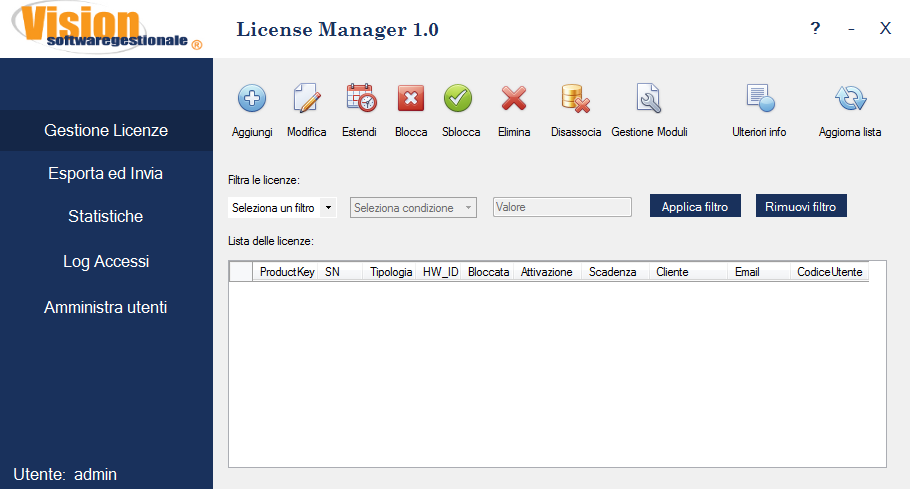
\includegraphics[width=1\columnwidth]{LicenseManager/primaSchermata} 
    \caption{Prima schermata all'avvio - Gestione Licenze}
    \label{primscher}
\end{figure}

Nella sezione “Gestione Licenze“ è possibile gestire tutti gli aspetti delle licenze.
Nello specifico le operazioni permesse, nell'ordine, sono:
\begin{itemize}
\item \textbf{Aggiungi:} permette di creare una nuova licenza;
\item modifica;
\item estensione della data di scadenza;
\item bloccaggio;
\item ecc....
\end{itemize} 
Nella parte alta della schermata sono presenti le funzionalità, mentre nella parte bassa è mostrata la lista delle licenze visibili all’utente, quindi tutte in caso di utente Admin, quelle con Codice Utente uguale al proprio codice in caso di utente Guest. In seguito sono mostrate nel dettaglio tutte le funzionalità. 

\subsection{Aggiungi}
La funzione “Aggiungi” permette di creare una nuova licenza. Il metodo di creazione differisce per gli utenti Admin e gli utenti Guest. Cliccando sul pulsante si apre una nuova finestra, dove è possibile inserire i dati di una licenza. La finestra è riportata nella Figura \ref{crealic}.

\begin{figure}[!h] 
    \centering 
    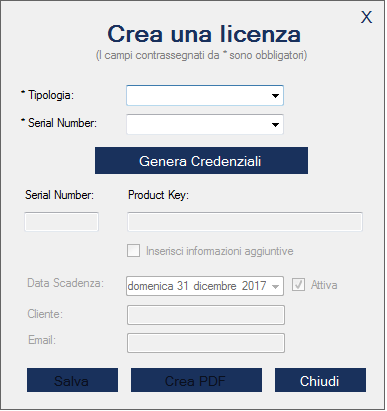
\includegraphics[width=0.7\columnwidth]{LicenseManager/creaLicenza} 
    \caption{Finestra Aggiungi - Gestione Licenze}
    \label{crealic}
\end{figure}

Per creare una licenza è necessario innanzitutto valorizzare i campi obbligatori, ovvero Tipologia e Serial Number. 
\begin{itemize}

\item \textbf{Tipologia:} Identifica quale licenza si sta creando, e i valori possibili sono SQL, LT, ERP o Trasporti. 
\item \textbf{Serial Number:} Numero di sei cifre che identifica in modo univoco, per tipologia, una licenza. Uno stesso Serial Number è permesso per diverse tipologie. La scelta del Serial Number differisce da Admin e Guest.  
\begin{itemize}

\item	\textbf{Admin:} Può scegliere tra un Serial Number “Manuale”, ossia sceglierlo direttamente senza limitazioni, “Casuale”, ossia viene creato un Serial Number casuale, “Prime due cifre per l’anno”, ossia le prime due cifre identificano l’anno di creazione, mentre le altre quattro identificano il punto di partenza da cui cercare un Serial Number libero.
\item	\textbf{Guest:} Può creare solo un Serial Number di tipologia “Prime due cifre per l’anno”.
\end{itemize}

\end{itemize}	

Dopo aver scelto Tipologia e Serial Number è necessario cliccare su “Genera Credenziali” per poter continuare con la creazione della licenza. Cliccando su questo pulsante è invocato un metodo del Web Service \texttt{License Manager Service} che produrrà un Serial Number compatibile con la scelta effettuata e un Product Key, che identifica univocamente una licenza, indipendentemente dalla tipologia. Qualora il Serial Number scelto in caso di selezione “Manuale “ o “Casuale” fosse già in uso, sarà comunicato che non è possibile utilizzare tali valori ed è necessario sceglierne degli altri. In caso di scelta “Prime due cifre per l’anno” il Serial Number prodotto sarà il primo libero disponibile a partire dal numero a quattro cifre scelto. Dopo la creazione delle credenziali il pulsante “Salva” si attiverà e sarà possibile salvare la licenza. 


%**************************************************************

\section{Esporta ed Invia}

%**************************************************************
\section{Statistiche}


%**************************************************************
\section{Log Accessi}


%**************************************************************
\section{Amministra Utenti}

